\subsection{Περιβάλλον υλοποίησης}

\subsubsection{Unity Editor}

\textbf{Εγκατάσταση}

Η εγκατάσταση του Unity Editor γίνεται μέσω του Unity Hub, το οποίο είναι μια αυτόνομη εφαρμογή με σκοπό την πρόσβαση στο οικοσύστημα Unity. Το Hub προσφέρει εύκολη διαχείριση των Unity projects και των αδειών για τα Unity λογισμικά, καθώς και προσφέρει τη δυνατότητα εγκατάστασης πρόσθετων στοιχείων (add-ons) και πολλών εκδόσεων του Unity Editor.

\begin{figure}[H]
    \centering
    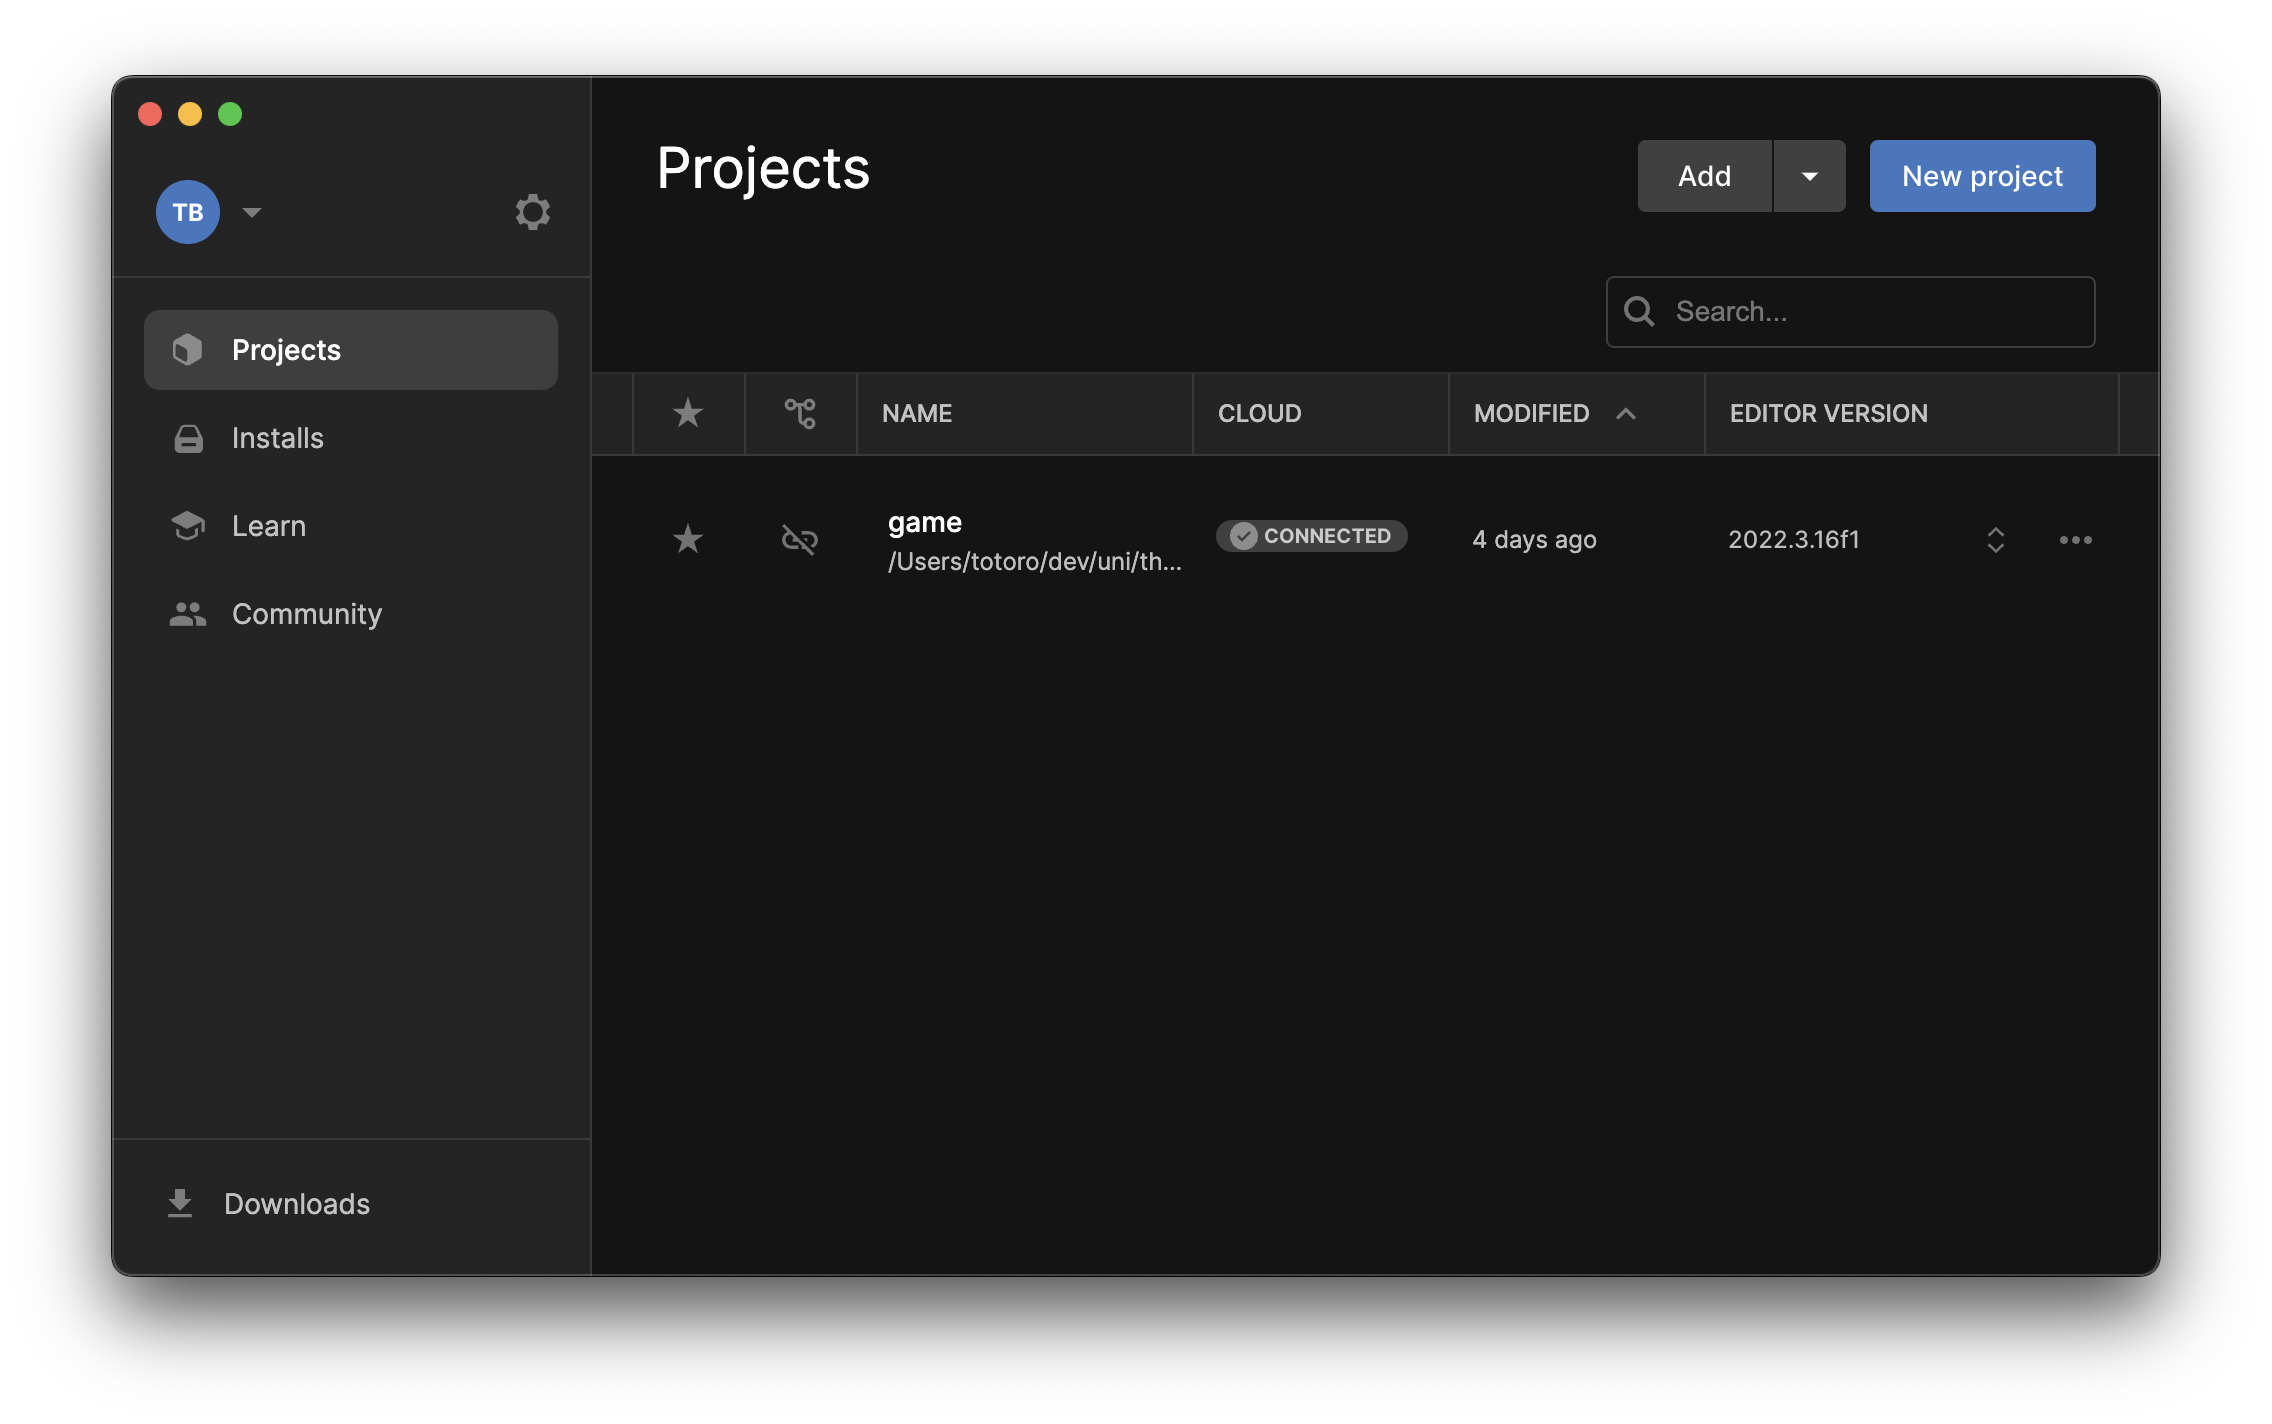
\includegraphics[width=1\linewidth]{sections/4/1/images/unity_hub}
    \caption{Το Unity Hub}
    \label{fig:unity_hub}
\end{figure}

\pagebreak
\showheader

Για τη δημιουργία του παιχνιδιού επιλέχθηκε το Unity Editor 2022.3.16f1 διότι ήταν η τελευταία τότε έκδοση \acrshort{lts}.

\textbf{Πρώτη ματιά}

Το Unity Editor προσφέρει μία φιλική προς το χρήστη διεπαφή η οποία αποτελείται από πολλά παράθυρα με διάφορους σκοπούς τα οποία μπορούν να τοποθετηθούν και να αποσυνδεθούν κατά βούληση. Αυτό προσφέρει τη δυνατότητα στο κάθε χρήστη να τα τοποθετήσει όπως εκείνος επιθυμεί.

\begin{figure}[H]
    \centering
    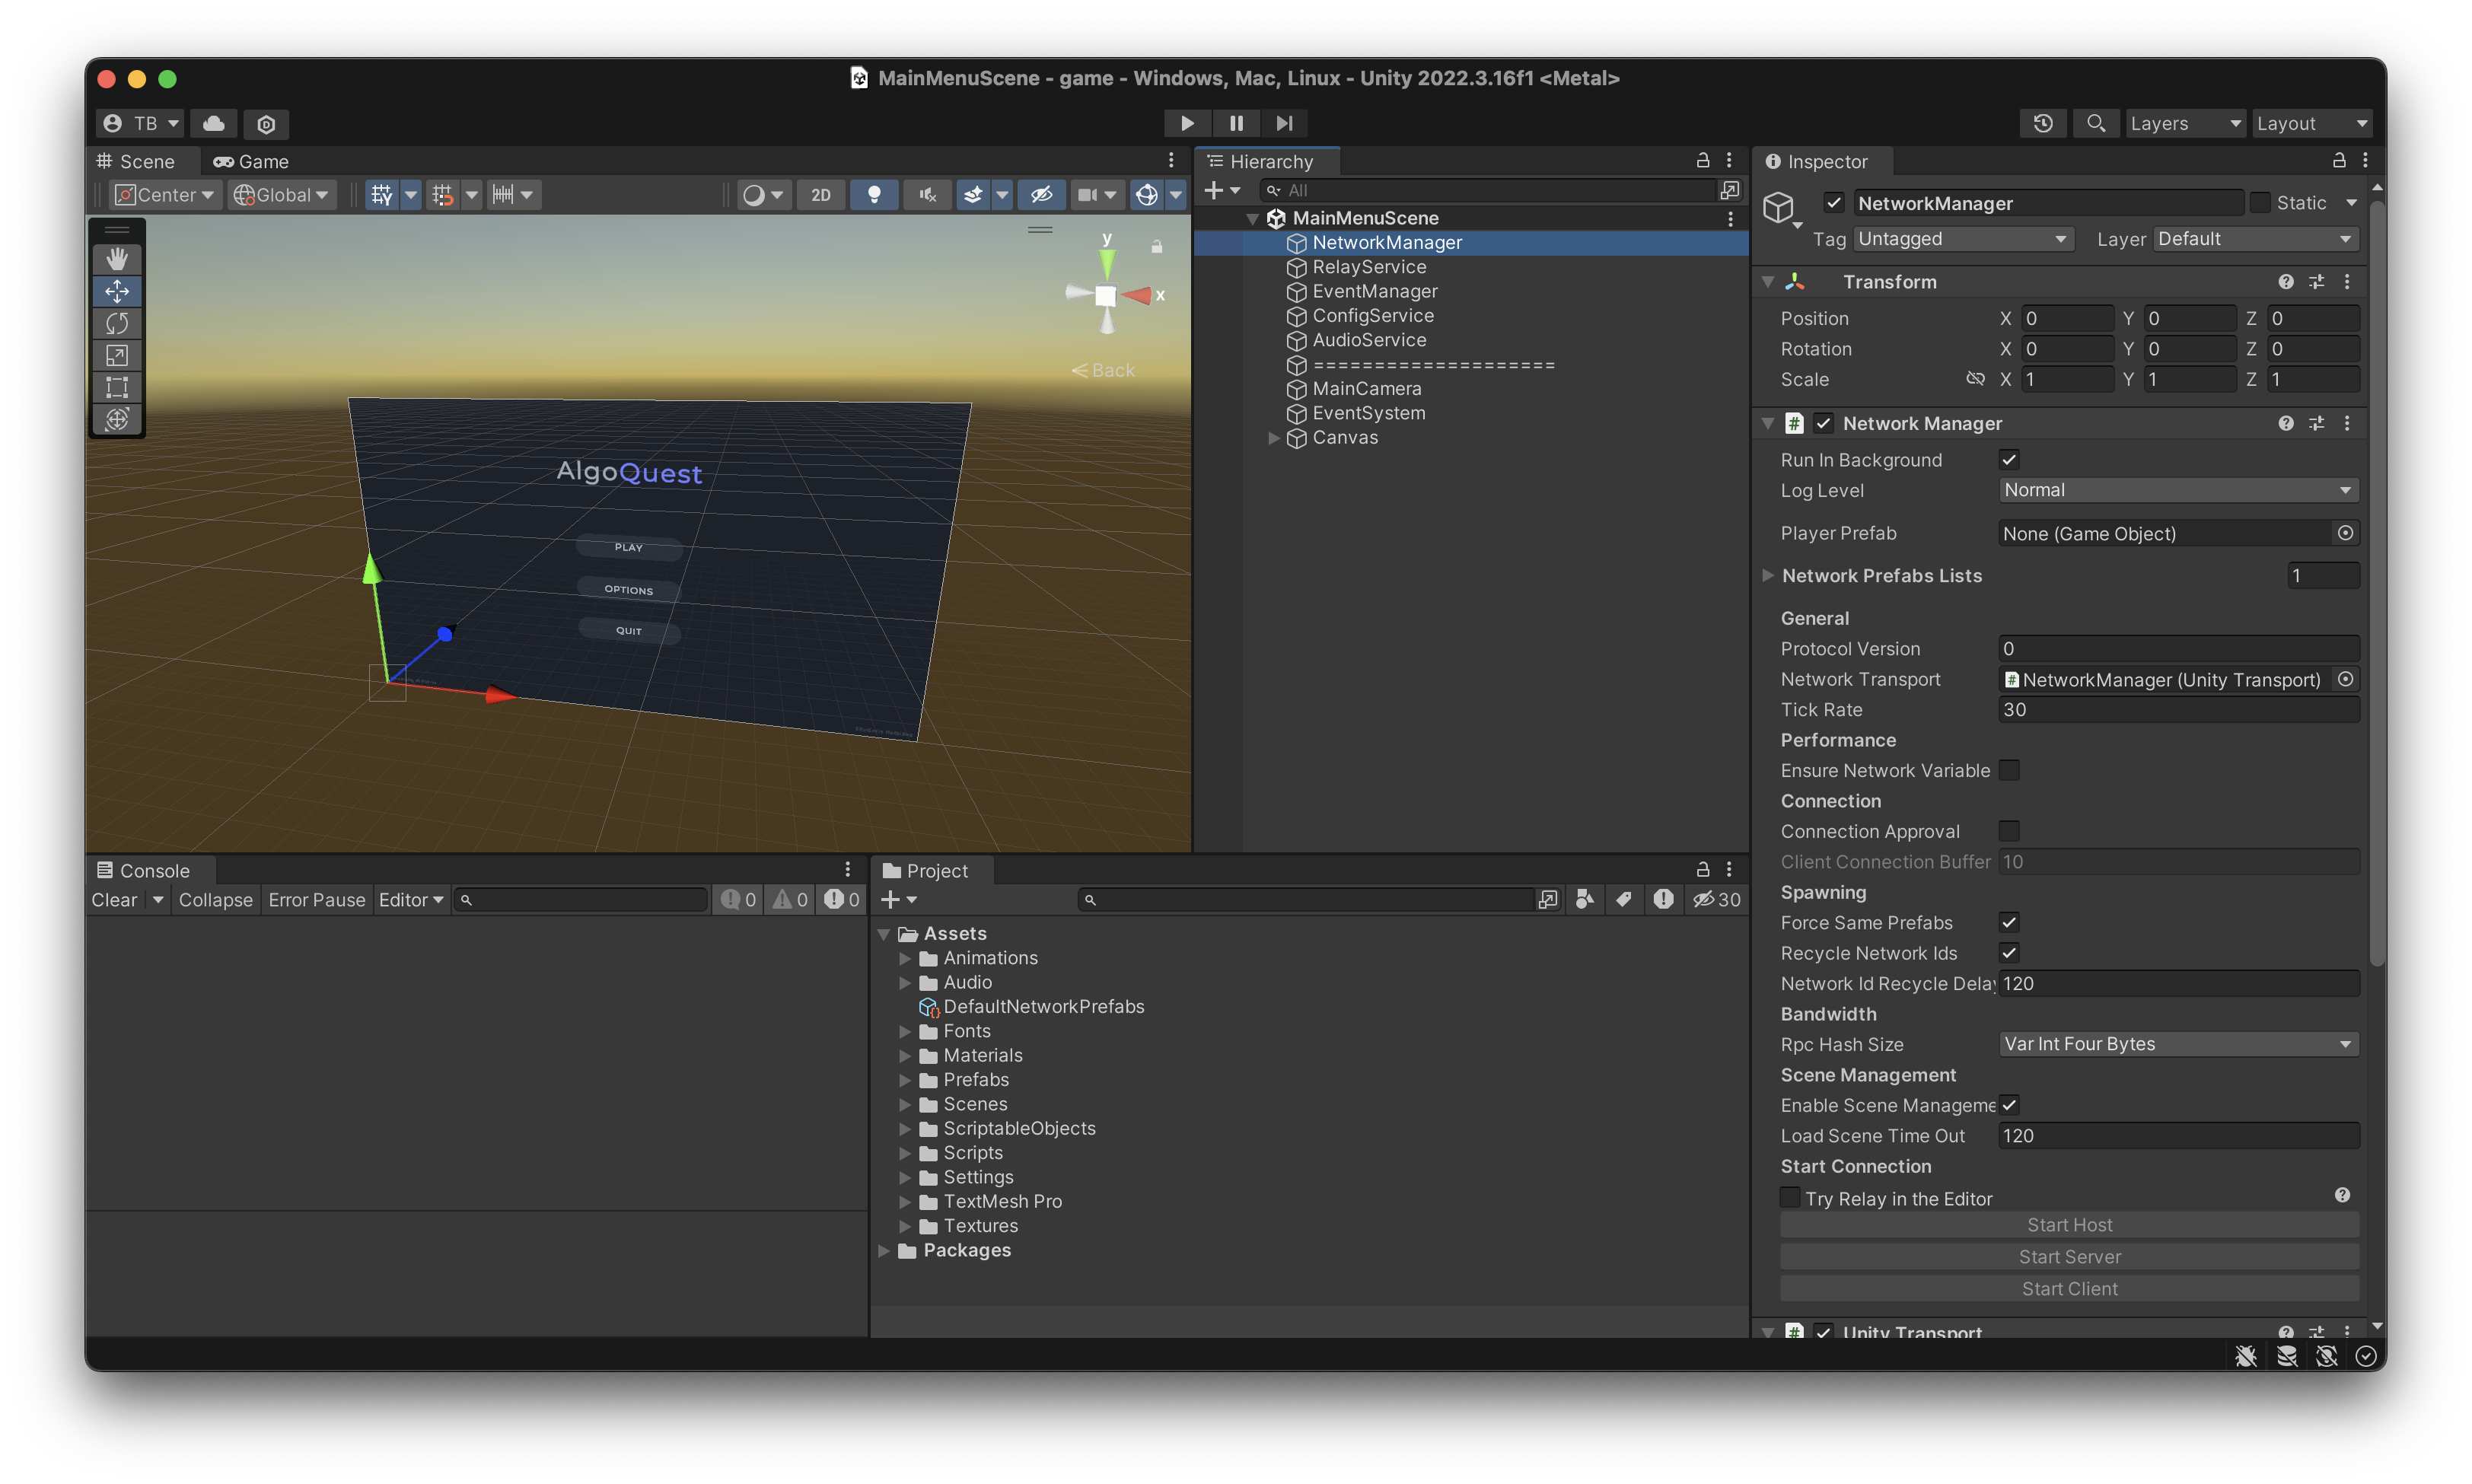
\includegraphics[width=1\linewidth]{sections/4/1/images/unity_editor}
    \caption{Το Unity Editor}
    \label{fig:unity_editor}
\end{figure}

Τα παράθυρα που προσφέρει το Unity Editor είναι αρκετά για να καλύψουν κάθε ανάγκη που μπορεί να έχει κάποιος ο οποίος θέλει να κατασκευάσει ένα παιχνίδι χρησιμοποιώντας την εφαρμογή. Από αυτά τα βασικότερα που χρησιμοποιήθηκαν κατά την κατασκευή αυτού του παιχνιδιού είναι τα εξής:

\begin{itemize}
    \item \textbf{Hierarchy (Εικόνα \ref{fig:unity_editor} πάνω-κέντρο):} Το παράθυρο αυτό περιέχει μία ιεραρχική μορφή όλων των GameObjects που υπάρχουν στην επιλεγμένη σκηνή. Ο χρήστης μπορεί να μετακινήσει κάποιο GameObject σε οποιοδήποτε μέρος του δέντρου επιθυμεί.
    \item \textbf{Scene (Εικόνα \ref{fig:unity_editor} πάνω-αριστερά):} Αυτό είναι το παράθυρο τρισδιάστατης προβολής του κόσμου το οποίο μπορεί να χρησιμοποιήσει ο χρήστης για να μετακινηθεί, καθώς και να ελέγξει τον κόσμο και τα GameObjects που βρίσκονται μέσα σε αυτόν.
    \item \textbf{Inspector (Εικόνα \ref{fig:unity_editor} δεξιά):} Αναμφισβήτητα το πιο σημαντικό παράθυρο του Unity Editor, το Inspector εμφανίζει όλα τα Components του επιλεγμένου GameObject. Με τη χρήση αυτών των components ο χρήστης μπορεί να διαχειριστεί την θέση του GameObject στον κόσμο, αλλά και την συμπεριφορά του σε αυτόν.
    \item \textbf{Console (Εικόνα \ref{fig:unity_editor} κάτω-αριστερά):} Σε αυτό το παράθυρο εμφανίζονται όλα τα logs της εφαρμογής κατά τη διάρκεια της κατασκευής, τα οποία μπορεί να είναι είτε λάθη που μπορεί να συμβούν στο παιχνίδι, είτε logs που ο ίδιος ο χρήστης έχει τοποθετήσει στον κώδικα του.
    \item \textbf{Project (Εικόνα \ref{fig:unity_editor} κάτω-κέντρο):} Εδώ εμφανίζονται όλα τα αρχεία που υπάρχουν στους φακέλους του project, είτε του ίδιου του χρήστη (φάκελος Assets) είτε του Unity και των πρόσθετων πακέτων που μπορεί να έχει κατεβάσει ο χρήστης (φάκελος Packages).
\end{itemize}

Σε αυτό το σημείο είναι σημαντικό να σημειωθεί πως το Unity Editor και τα παράθυρα του είναι μία συλλογή από scripts. Αυτό σημαίνει, πως εκτός από τη συνηθισμένη χρήση των scripts που γράφει ένας χρήστης, τα οποία αφορούν την συμπεριφορά των GameObjects στον κόσμο, μπορεί κάποιος να γράψει scripts τα οποία δημιουργούν παράθυρα για κάποιο ειδικό σκοπό. Οι πιθανές χρήσεις τους μπορεί να είναι σχετικά απλές, όπως η δημιουργία παραθύρου για \glspl{cheat_code} ή αρκετά περίπλοκες, όπως για τον έλεγχο της συμπεριφοράς GameObject σε κάποιο cutscene όπως βλέπουμε στην εικόνα \ref{fig:unity_custom_editor_windows}\cite{technologies_unity_nodate}.

\begin{figure}[H]
    \centering
    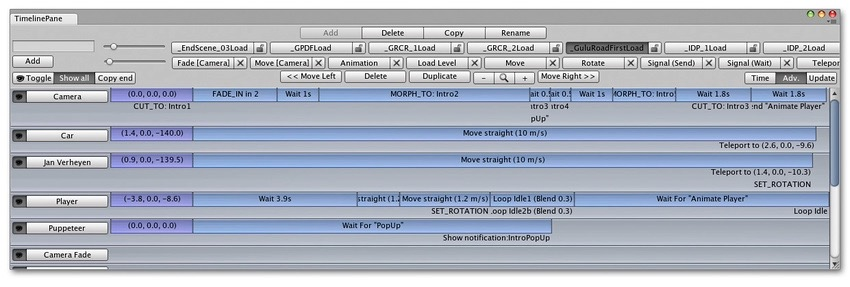
\includegraphics[width=1\linewidth]{sections/4/1/images/unity_custom_editor_windows}
    \caption{Unity παράθυρο ειδικού σκοπού που χρησιμοποιείται για τον έλεγχο της συμπεριφοράς GameObject σε cutscene}
    \label{fig:unity_custom_editor_windows}
\end{figure}

\textbf{Scenes}

Η κατασκευή εφαρμογών στο Unity γίνεται με τη χρήση σκηνών (Scenes), όπου κάθε σκηνή είναι ένα ξεχωριστό επίπεδο ή περιβάλλον μέσα στο project. Σε αυτές τοποθετούνται διάφορα GameObjects όπως χαρακτήρες, φωτισμός και κάμερες τα οποία μπορούν να ρυθμιστούν και να αλληλεπιδρούν μέσα σε αυτές τις σκηνές.

Χρησιμεύουν επίσης ως δοχεία από GameObjects τα οποία κάνουν εύκολη την οργάνωση και σχεδίαση του κόσμου μιας εφαρμογής, καθώς μοιράζουν τον εικονικό κόσμο σε εύκολα διαχειρίσιμα τμήματα.

Λόγω της αρθρωτής φύσης τους, οι σκηνές διευκολύνουν τις ομαλές μεταβάσεις μεταξύ διαφορετικών τμημάτων μιας εφαρμογής, όπως η πλοήγηση από ένα μενού σε ένα περιβάλλον παιχνιδιού.

\textbf{GameObjects}

Το θεμελιώδες δομικό στοιχείο μιας εφαρμογής στο Unity, το GameObject, αντιπροσωπεύει μία οντότητα σε μία σκηνή. Κάθε στοιχείο σε μία σκηνή, είτε πρόκειται για χαρακτήρα, είτε για σκηνικό, είτε για περιβαλλοντικό χαρακτηριστικό, είναι μία περίπτωση ενός GameObject. Με διάφορους συνδυασμούς Components μπορούν να μετατραπούν σε οτιδήποτε, από ένα φόντο σε ένα μενού μέχρι έναν πολύπλοκο και διαδραστικό χαρακτήρα παίκτη.

Το Unity προσφέρει μια εναλλακτική λύση για υλοποίηση εφαρμογής αντί για GameObjects, το \acrfull{unity_ecs}\cite{noauthor_entity_nodate}, μέρος του \acrfull{unity_dots} του Unity\cite{noauthor_dots_nodate}, το οποίο έχει μεγαλύτερο προσανατολισμό στην απόδοση. Τα Entities είναι ελαφριά δοχεία δεδομένων τα οποία διαχωρίζουν τα δεδομένα και τη συμπεριφορά ενός αντικειμένου, με σκοπό τη μεγιστοποίηση της αποδοτικότητας του χρόνου εκτέλεσης και την καλύτερη χρήση των επεξεργαστών με πολλαπλούς πυρήνες. Η χρήση τους, δυστυχώς, δεν είναι τόσο διαδεδομένη όσο των GameObjects με αποτέλεσμα να υπάρχουν λιγότεροι πόροι βοήθειας, καθώς και χαμηλότερη υποστήριξη από την κοινότητα του Unity. Αυτός είναι και ο λόγος για τον οποίο επιλέχθηκαν τα GameObjects για αυτή την εφαρμογή.

\textbf{Components}

Τα Components είναι βασικά στοιχεία τα οποία τοποθετούνται σε GameObjects και καθορίζουν τη συμπεριφορά, την εμφάνιση και τη λειτουργικότητα τους. Είναι αυτά που δίνουν στα GameObjects τις ξεχωριστές τους ιδιότητες και δυνατότητες μέσα σε ένα Scene.

Υπάρχουν διάφοροι τύποι Components που μπορούν να χρησιμοποιηθούν στα GameObjects, όπως:

\begin{itemize}
    \item \textbf{Transform Components:} Κάθε GameObject περιλαμβάνει εξ ορισμού ένα Component Transform, το οποίο καθορίζει τη θέση, την περιστροφή και την κλίμακα του GameObject στο Scene.
    \item \textbf{Physical Components:} Περιλαμβάνουν Rigidbody και Colliders που επιτρέπουν αλληλεπιδράσεις βασισμένες στη φύση, όπως η βαρύτητα και οι συγκρούσεις.
    \item \textbf{Visual Components:} Μπορεί να είναι Mesh Renderer Components, τα οποία είναι υπεύθυνα για την εμφάνιση των μοντέλων των GameObjects, ή ακόμη και Light Components τα οποία επηρεάζουν τον φωτισμό και τις σκιές.
    \item \textbf{Audio Components:} Audio Source ή Audio Listener Components τα οποία χρησιμοποιούνται για την αναπαραγωγή ήχων και τη διαχείριση του τρόπου με τον οποίο ο ήχος γίνεται αντιληπτός στο περιβάλλον.
    \item \textbf{Scripts:} Κώδικες γραμμένοι συνήθως σε C\#\cite{noauthor_c_nodate}, μπορούν να προστεθούν ως Components για τον έλεγχο της συμπεριφοράς των GameObject μέσω κώδικα.
\end{itemize}

\textbf{Scripts}

Τα Script μπορούν να χρησιμοποιηθούν για τον έλεγχο της εφαρμογής μέσω κώδικα. Συνήθως γραμμένα σε C\#, μπορούν είτε να προστεθούν σε Components εφόσον κληρονομούν από την κλάση \verb|MonoBehaviour| που παρέχει το Scripting API του Unity (ή την \verb|NetworkBehaviour| εφόσον χρειάζεται λειτουργικότητα στο δίκτυο), είτε σαν δεδομένα που μπορούν να μοιράζονται μεταξύ πολλών Script, εφόσον κληρονομούν από την κλάση \verb|ScriptableObject|, είτε να χρησιμοποιηθούν σαν απλά Scripts που προσφέρουν παραπάνω λειτουργικότητα σε άλλα Script, όπως το να επικοινωνούν με εξωτερικές υπηρεσίες.

Τα Scripts που κληρονομούν από την κλάση \verb|MonoBehaviour| προσφέρουν τη δυνατότητα να επικοινωνούν με το Unity Editor και να διαχειρίζονται τη συμπεριφορά των GameObjects.
\begin{itemize}
    \item \textbf{Event functions:} Συναρτήσεις συμβάντων που συμβαίνουν σε διαφορετικά στάδια της ζωής μιας εφαρμογής. Μερικές από αυτές είναι:
    \begin{itemize}
        \item \verb|OnEnable()| και \verb|OnDisable()|: Καλούνται όταν το GameObject ενεργοποιείται ή απενεργοποιείται αντίστοιχα.
        \item \verb|Awake()|: Καλείται όταν το GameObject δημιουργείται.
        \item \verb|Start()|: Καλείται πριν το πρώτο καρέ της εφαρμογής.
        \item \verb|Update()|: Καλείται κάθε καρέ της εφαρμογής.
    \end{itemize}
    \item \textbf{Coroutines:} Είναι μέθοδοι οι οποίες μπορούν να διακόψουν την εκτέλεση του Script και να επιστρέψουν τον έλεγχο στο Unity, αλλά στη συνέχεια να συνεχίσουν από εκεί που σταμάτησαν σε επόμενα καρέ.
    \item \textbf{Physics events:} Μέθοδοι συμβάντων οι οποίες μπορούν να χρησιμοποιηθούν για το χειρισμό της φυσικής και των συγκρούσεων. Οι βασικότερες από αυτές, \verb|OnCollisionEnter()| και \verb|OnTriggerEnter()|, ανταποκρίνονται στις αλληλεπιδράσεις της φυσικής αν το GameObject έχει κάποιο Collider Component.
    \item \textbf{Messaging system:} Η κλάση \verb|MonoBehaviour| περιλαμβάνει ένα σύστημα μυνημάτων, το οποίο επιτρέπει σε Scripts να στέλνουν και να λαμβάνουν μηνύματα που μπορούν να καλέσουν μεθόδους. Συναρτήσεις όπως \verb|SendMessage()| και \verb|BroadcastMessage()| επιτρέπουν αυτή την επικοινωνία μεταξύ Scripts.
    \item \textbf{Lifecycle control:} Περιλαμβάνει μεθόδους που μπορούν να χρησιμοποιηθούν για τον έλεγχο της ζωής του GameObject, όπως \verb|Destroy()| η οποία καταστρέφει ένα GameObject από ένα Scene ή \verb|OnDestroy()| που καλείται όταν το GameObject καταστρέφεται.
    \item \textbf{Editor control:} Scripts που κληρονομούν από την κλάση \verb|MonoBehaviour| μπορούν να εμφανίσουν πεδία στο Unity Editor τα οποία αντιστοιχούν σε μεταβλητές μέσα στα αντίστοιχα Script. Αυτό επιτρέπει τον έλεγχο και τη ρύθμιση παραμέτρων του GameObject χωρίς να χρειάζεται να χτιστεί κάθε φορά το Script, καθώς και εύκολο έλεγχο του GameObject από άτομα τα οποία δεν έχουν γνώσεις σε γλώσσες προγραμματισμού.
\end{itemize}

\begin{figure}[H]
    \centering
    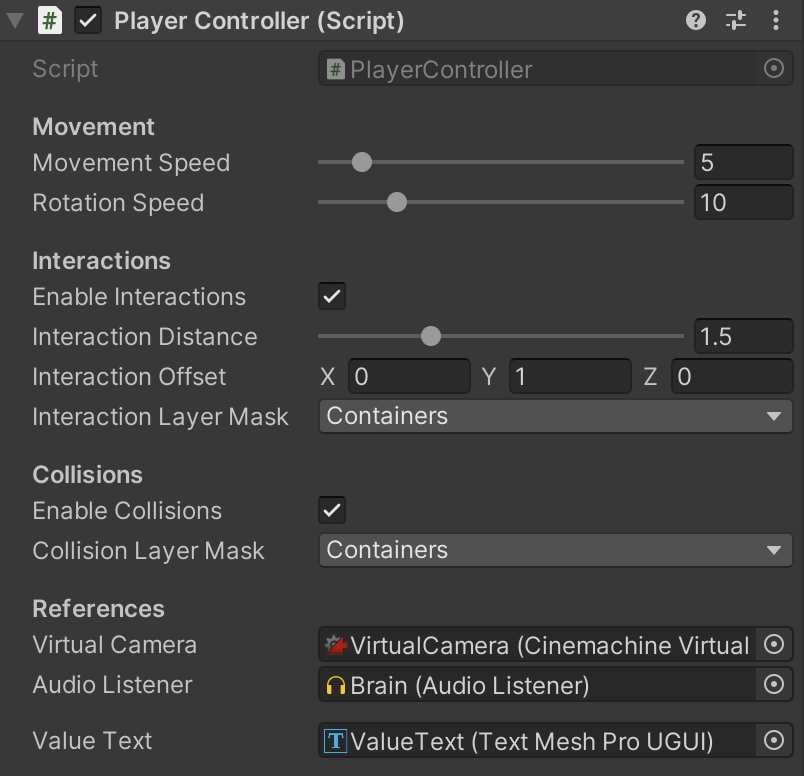
\includegraphics[width=0.6\linewidth]{sections/4/1/images/unity_editor_player_controller}
    \caption{Script ελέγχου του παίκτη με πεδία στο Unity Editor}
    \label{fig:unity_editor_player_controller}
\end{figure}

Τα Scripts που κληρονομούν από την κλάση \verb|ScriptableObject| επιτρέπουν στους χρήστες να δημιουργούν αντικείμενα τα οποία δεν χρειάζεται να είναι συνδεδεμένα με κάποιο GameObject. Παρέχουν ένα τρόπο αποθήκευσης δεδομένων ανεξάρτητο από Scenes ή GameObjects, προσφέροντας έτσι έναν εύκολο τρόπο διαχείρισης κοινών δεδομένων σε μία εφαρμογή.

Ένα ακόμη καλό των \verb|ScriptableObject| είναι πως δημιουργούνται μέσω του \gls{context_menu} προσφέροντας έτσι έναν εύκολο τρόπο σε χρήστες που δεν έχουν γνώσεις στον προγραμματισμό να διαχειριστούν την εφαρμογή.

Συγχρόνως προσφέρουν οργάνωση και αποδοτικότητα καθώς αποθηκεύονται σε ένα σημείο και όχι σε κάθε GameObject οπότε μειώνουν τον χώρο αποθήκευσης που χρειάζεται κάποιος για την εφαρμογή, καθώς και προσφέρουν ένα κεντρικό σημείο από το οποίο μπορεί κάποιος να ρυθμίσει μεταβλητές της εφαρμογής. Αυτό μπορεί να συμβεί και κατά τη διάρκεια του παιχνιδιού στο Unity Editor, κάτι το οποίο δεν ισχύει για τις ρυθμίσεις πάνω σε ένα GameObject.

\begin{figure}[H]
    \centering
    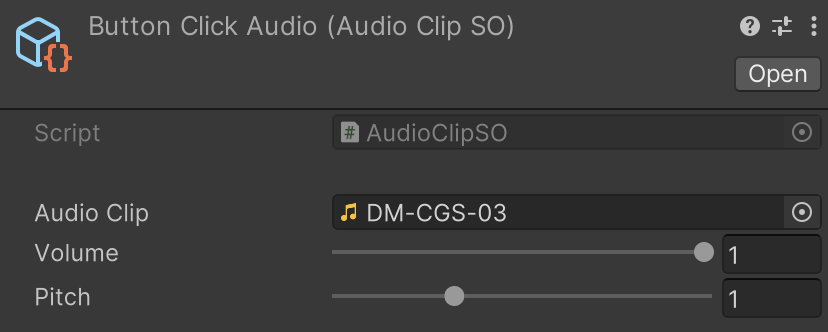
\includegraphics[width=0.6\linewidth]{sections/4/1/images/unity_editor_button_click_audio_so}
    \caption{ScriptableObject για τον έλεγχο του ήχου που παίζει όταν κάποιος παίκτης κάνει κλικ σε ένα κουμπί}
    \label{fig:unity_editor_button_click_audio_so}
\end{figure}

% ========================================

\subsubsection{REST API Server}

Κατά τον σχεδιασμό του παιχνιδιού υπήρξε η ανάγκη να μπορεί ο εκπαιδευτικός με κάποιο τρόπο να συλλέξει δεδομένα και στατιστικά για την πρόοδο των παικτών σε αυτό, καθώς και να ρυθμίσει παραμέτρους του. Χρειάστηκε λοιπόν κάποια δομή αποθήκευσης δεδομένων η οποία θα βρισκόταν σε ένα κεντρικό σημείο με το οποίο θα μπορούσε να αλληλεπιδρά ο εκπαιδευτικός. Μία βάση δεδομένων είναι ο τέλειος υποψήφιος για αυτό που απαιτείται, αλλά ένα παιχνίδι Unity δεν έχει τη δυνατότητα να αλληλεπιδρά απευθείας με μια βάση δεδομένων.

\acrlong{rest} \acrlong{api}, πιο γνωστό ως \acrshort{rest} \acrshort{api}\cite{noauthor_what_nodate-1} είναι ένα σύνολο κανόνων και πρωτοκόλλων με σκοπό τη δημιουργία και αλληλεπίδραση με διαδικτυακές υπηρεσίες. Επιτρέπουν σε διάφορα συστήματα λογισμικού να επικοινωνούν μέσω του διαδικτύου με τη χρήση μεθόδων \acrshort{http} όπως GET, POST και DELETE\cite{noauthor_http_2023}. Είναι σχεδιασμένα έτσι ώστε να είναι \gls{stateless}, δηλαδή κάθε αίτημα που εκτελεί ένας χρήστης περιέχει όλες τις πληροφορίες που χρειάζεται ο \gls{server} για να το ικανοποιήσει.

Χρησιμοποιώντας τον συνδυασμό μιας βάσης δεδομένων και ενός \acrshort{rest} \acrshort{api} λοιπόν, μπορεί να δημιουργηθεί μία διεπαφή με την οποία θα επικοινωνούν όλοι οι παίκτες του παιχνιδιού. Αυτό δίνει πια τη δυνατότητα να αποθηκεύονται δεδομένα και στατιστικά για τις αλληλεπιδράσεις τους μέσα στον εικονικό κόσμο.

\textbf{Βάση δεδομένων}

Κατά την επιλογή βάσης δεδομένων, το πρώτο εμπόδιο που εμφανίστηκε ήταν ή επιλογή μεταξύ σχεσιακής (\acrshort{sql}\cite{noauthor_what_nodate-2}) ή μή (\acrshort{nosql}\cite{noauthor_what_nodate-3}) βάσης. Παρότι τα δεδομένα τα οποία συνήθως αποθηκεύονται για ένα παιχνίδι είναι μη δομημένα, κάτι το οποίο ακούγεται πράγματι ιδανικό για μη-σχεσιακές βάσεις, στη περίπτωση αυτή τα δεδομένα εμφανίζονται πιο πολύ σε μορφή αρχείων καταγραφής από οτιδήποτε άλλο. Το γεγονός αυτό, σε συνδυασμό με το ότι τα δεδομένα σε μία σχεσιακή βάση δεδομένων είναι πιο εύκολα κατανοητά από ανθρώπους, οδήγησε στην επιλογή \acrshort{sql} βάσης.

Το επόμενο βήμα ήταν η επιλογή συστήματος διαχείρισης σχεσιακών βάσεων \acrfull{rdbms}, και στο σταυροδρόμι αυτό οι επιλογές που εμφανίστηκαν ήταν η MySQL\cite{noauthor_mysql_nodate} και η PostgreSQL\cite{group_postgresql_2024}. Παρότι η MySQL χρησιμοποιείται ευρέως και θεωρείται από τα καλύτερα συστήματα, οι περισσότερες επιλογές τύπων δεδομένων της PostgreSQL, μαζί με την καλύτερη απόδοση σε εγγραφές, καθώς και το γεγονός πως είναι η επιλογή που προτιμούν οι επαγγελματίες\cite{noauthor_stack_nodate}, οδήγησε στην επιλογή της. Καθώς ο αριθμός των παικτών που θα δημιουργούν εγγραφές στη βάση είναι πολύ πιο μεγάλος από τους χρήστες που θα διαβάζουν τα δεδομένα της, ήταν σημαντική η επιλογή της PostgreSQL καθώς έχει καλύτερη απόδοση σε εγγραφές σε σχέση με τη MySQL.

Η εγκατάσταση της βάσης δεδομένων ήταν πιθανώς η πιο εύκολη διαδικασία, καθώς το Docker\cite{noauthor_docker_nodate}, μία πλατφόρμα που έχει σχεδιαστεί για την ανάπτυξη και την εκτέλεση εφαρμογών σε \glspl{docker_container}, είναι το τέλειο εργαλείο για αυτή τη περίπτωση. Το \gls{docker_image} της PostgreSQL που προσφέρει η ομάδα της, αναβαθμίζεται συχνά και είναι εγγυημένο πως θα λειτουργήσει σε κάθε σύστημα που μπορεί να εγκατασταθεί, αφού είναι συσκευασμένη μαζί με όλα τα παρελκόμενα που χρειάζεται.

\textbf{API}

Η κατασκευή του \acrshort{api} αποτελεί βασικό μέρος του παιχνιδιού καθώς θα είναι η διεπαφή με την οποία θα επικοινωνεί το παιχνίδι, καθώς και οποιαδήποτε άλλη εξωτερική εφαρμογή επιθυμεί πρόσβαση στα δεδομένα της βάσης.

Η τεχνολογία \acrshort{rest} \acrshort{api} είναι αρκετά συχνή στις μέρες μας, καθώς χρησιμοποιείται από τις περισσότερες διαδικτυακές εφαρμογές και όχι μόνο. Είναι λοιπόν λογικό να υπάρχουν μέθοδοι υλοποίησης ενός \acrshort{rest} \acrshort{api} σε διάφορες πλατφόρμες και συστήματα. Από αυτές, ξεχωρίζει το Node.js\cite{noauthor_nodejs_nodate}, το δημοφιλέστερο \gls{js_runtime} για backend \acrshort{api}. Είναι βασισμένο στη μηχανή V8 του Google Chrome\cite{noauthor_v8_nodate} η οποία κάνει χρήση της τεχνικής \acrshort{jit} compilation, και μεταγλωτίζει τον κώδικα προτού τον εκτελέσει, προσφέροντας έτσι πολύ καλή απόδοση.

Η υλοποίηση ενός \acrshort{rest} \acrshort{api} με Node.js γίνεται συνήθως με τη χρήση Express, ενός μινιμαλιστικού framework γραμμένο για Node.js που έχει έμφαση στην ταχύτητα και την απλότητα του. Στη περίπτωση αυτή όμως, υπήρξε η ανάγκη να μπορεί ο εκπαιδευτικός να διαχειριστεί διάφορες παραμέτρους του παιχνιδιού καθώς και να δει στατιστικά από τους παίκτες. Αυτό είναι σαφώς εφικτό μέσω της βάσης δεδομένων, αλλά άμεση παρέμβαση στα δεδομένα είναι όχι μόνο επικίνδυνο, καθώς μπορούν να συμβούν ανθρώπινα λάθη, αλλά και αδύνατο, διότι η βάση δεδομένων θα είναι προσβάσιμη μόνο από συγκεκριμένα δίκτυα σε \gls{prod_env}. Η λύση λοιπόν παρουσιάστηκε σε μορφή εφαρμογής η οποία θα μπορεί να επικοινωνήσει άμεσα με το \acrshort{rest} \acrshort{api}.

Next.js από την Vercel\cite{noauthor_nextjs_nodate}, είναι ένα React\cite{noauthor_react_nodate} \gls{framework} βασισμένο επάνω στο Node.js, το οποίο προσφέρει τη δυνατότητα υλοποίησης \acrshort{rest} \acrshort{api} και frontend εφαρμογής μαζί. Αυτό είναι κάτι πάρα πολύ χρήσιμο καθώς χρειάζεται συντήρηση του κώδικα σε ένα μόνο σημείο και γνώση μόνο μιας γλώσσας προγραμματισμού, οπότε και ήταν η πρώτη επιλογή για την υλοποίηση των υποστηρικτών εφαρμογών του παιχνιδιού.

Τα \glspl{endpoint} που υλοποιήθηκαν στο \acrshort{rest} \acrshort{api} είναι τα εξής:
\begin{itemize}
    \item \textbf{POST /api/sessions:} Δημιουργεί ένα νέο session στη βάση και επιστρέφει τα δεδομένα του στο παιχνίδι για επόμενα requests.
    \item \textbf{GET /api/time-trials:} Επιστρέφει τα καλύτερα Χ σκορ, όπου Χ παράμετρος του αιτήματος. Τα σκορ επιλέγονται με βάση τον αριθμό των κουτιών καθώς και τον κινήσεων που χρειάζονται.
    \item \textbf{POST /api/container-interactions:} Δημιουργεί μία νέα εγγραφή στη βάση που καταγράφει την αλληλεπίδραση ενός παίκτη με ένα κουτί.
    \item \textbf{POST /api/logs:} Δημιουργεί μία νέα εγγραφή στη βάση που καταγράφει κινήσεις του παίκτη στην εφαρμογή.
    \item \textbf{GET /api/algorithms:} Επιστρέφει τις ρυθμίσεις των αλγορίθμων που υπάρχουν στη βάση. Για χρήση από τους εκπαιδευτικούς μέσω του διαχειριστικού.
    \item \textbf{POST /api/algorithms:} Δημιουργεί μία νέα εγγραφή με ρυθμίσεις για αλγόριθμο στη βάση. Για χρήση από τους εκπαιδευτικούς μέσω του διαχειριστικού.
    \item \textbf{PUT /api/algorithms:} Ανανεώνει τις ρυθμίσεις ενός αλγόριθμου στη βάση. Για χρήση από τους εκπαιδευτικούς μέσω του διαχειριστικού.
    \item \textbf{GET /api/algorithms/[type]:} Επιστρέφει τις ρυθμίσεις για έναν αλγόριθμο για χρήση από το παιχνίδι. Το παιχνίδι διαβάζει αυτές κατά την εκκίνηση ενός κόσμου και δημιουργεί τα κουτιά και τις τιμές αντίστοιχα.
\end{itemize}

\textbf{Παραδοχές \& πιθανές βελτιώσεις}

Καθώς ο αριθμός των παράλληλων παικτών που αναμένεται να παίξει το παιχνίδι σε αυτή την εργασία δεν είναι πολύ μεγάλος, αποφασίστηκε, οι εγγραφές στην βάση να γίνονται απευθείας από το \acrshort{rest} \acrshort{api}. Αυτή η παραδοχή δεν είναι εφικτή σε \gls{prod_env} όπου ο αριθμός χρηστών θα είναι πολύ μεγαλύτερος, διότι η καθυστέρηση που θα υπήρχε μέχρι να ολοκληρώσουν οι παίκτες της εγγραφές τους στη βάση θα έδινε μία πολύ κακή εμπειρία χρήστη.

Την ίδια στιγμή, ο μεγαλύτερος όγκος δεδομένων στη βάση δεδομένων είναι από εγγραφές που καταγράφουν κινήσεις παικτών στο παιχνίδι, οι οποίες δεν χρησιμοποιούνται από την ίδια εφαρμογή, αλλά για συλλογή στατιστικών από τους εκπαιδευτές. Αυτό αυξάνει το κόστος και το χρόνο απόκρισης της βάσης δεδομένων χωρίς να έχει κάποιο αποτέλεσμα για τους παίκτες.

Μελλοντικά λοιπόν θα ήταν ιδανικό να υλοποιηθεί μία λύση για τα παραπάνω προβλήματα. Μία από αυτές θα ήταν ο συνδυασμός χρήσης ενός \gls{bucket} όπως ο S3 των \acrfull{aws}\cite{noauthor_amazon_nodate} μαζί με ένα \gls{data_pipeline} όπως το Firehose των \acrshort{aws}\cite{noauthor_amazon_nodate-1}, τα οποία θα αποθηκεύουν τα δεδομένα σαν αντικείμενα στο \gls{bucket}, χωρίς να εμπλέκεται καθόλου η βάση δεδομένων. Για την μείωση του κόστους θα ήταν ιδανική επίσης η χρήση ενός \gls{data_warehouse} όπως το Snowflake\cite{noauthor_snowflake_nodate}, με πολύ χαμηλό κόστος εγγραφών σε σχέση με παραδοσιακές βάσεις δεδομένων που απαιτείται ταχύτητα. Τα δεδομένα από τον κουβά θα συλλέγονταν με κάποια χρονική καθυστέρηση και θα καταγράφονταν στην αποθήκη για χρήση από τους εκπαιδευτικούς.

Καθώς το παιχνίδι είναι μια εφαρμογή που θα εγκαθίσταται στον υπολογιστή των παικτών, η αποθήκευση κρυφών και προστατευμένων δεδομένων είναι δύσκολη. Αυτό σημαίνει πως η επικοινωνία του με το \acrshort{rest} \acrshort{api} θα πρέπει να γίνει χωρίς προστασία των αιτημάτων. Δυστυχώς αυτό έχει ως αποτέλεσμα να μπορούν κακόβουλοι χρήστες να στέλνουν αιτήματα χωρίς να βρίσκονται μέσα στο παιχνίδι, κάτι που μπορεί πολύ εύκολα να προκαλέσει πρόβλημα στα συστήματα που χρησιμοποιούνται για το παιχνίδι.

Μελλοντικά θα ήταν ιδανικό να βρεθεί κάποια μέθοδος με την οποία το \acrshort{rest} \acrshort{api} θα δέχεται αιτήματα μόνο μέσω του παιχνιδιού και όχι από εξωτερικά συστήματα.

% ========================================

\subsubsection{Διαχειριστικό εκπαιδευτικών}\label{sssec:admin_dashboard}

Με σκοπό την πιό εύκολη διαχείριση και ρύθμιση των βασικών σημείων του παιχνιδιού, καθώς και την προβολή στατιστικών, δημιουργήθηκε ένα βασικό διαχειριστικό στο οποίο έχουν πρόσβαση οι εκπαιδευτικοί. Αυτή η πλατφόρμα σερβίρεται από τον ίδιο \gls{server} με τη βοήθεια του Next.js.

\begin{figure}[H]
    \centering
    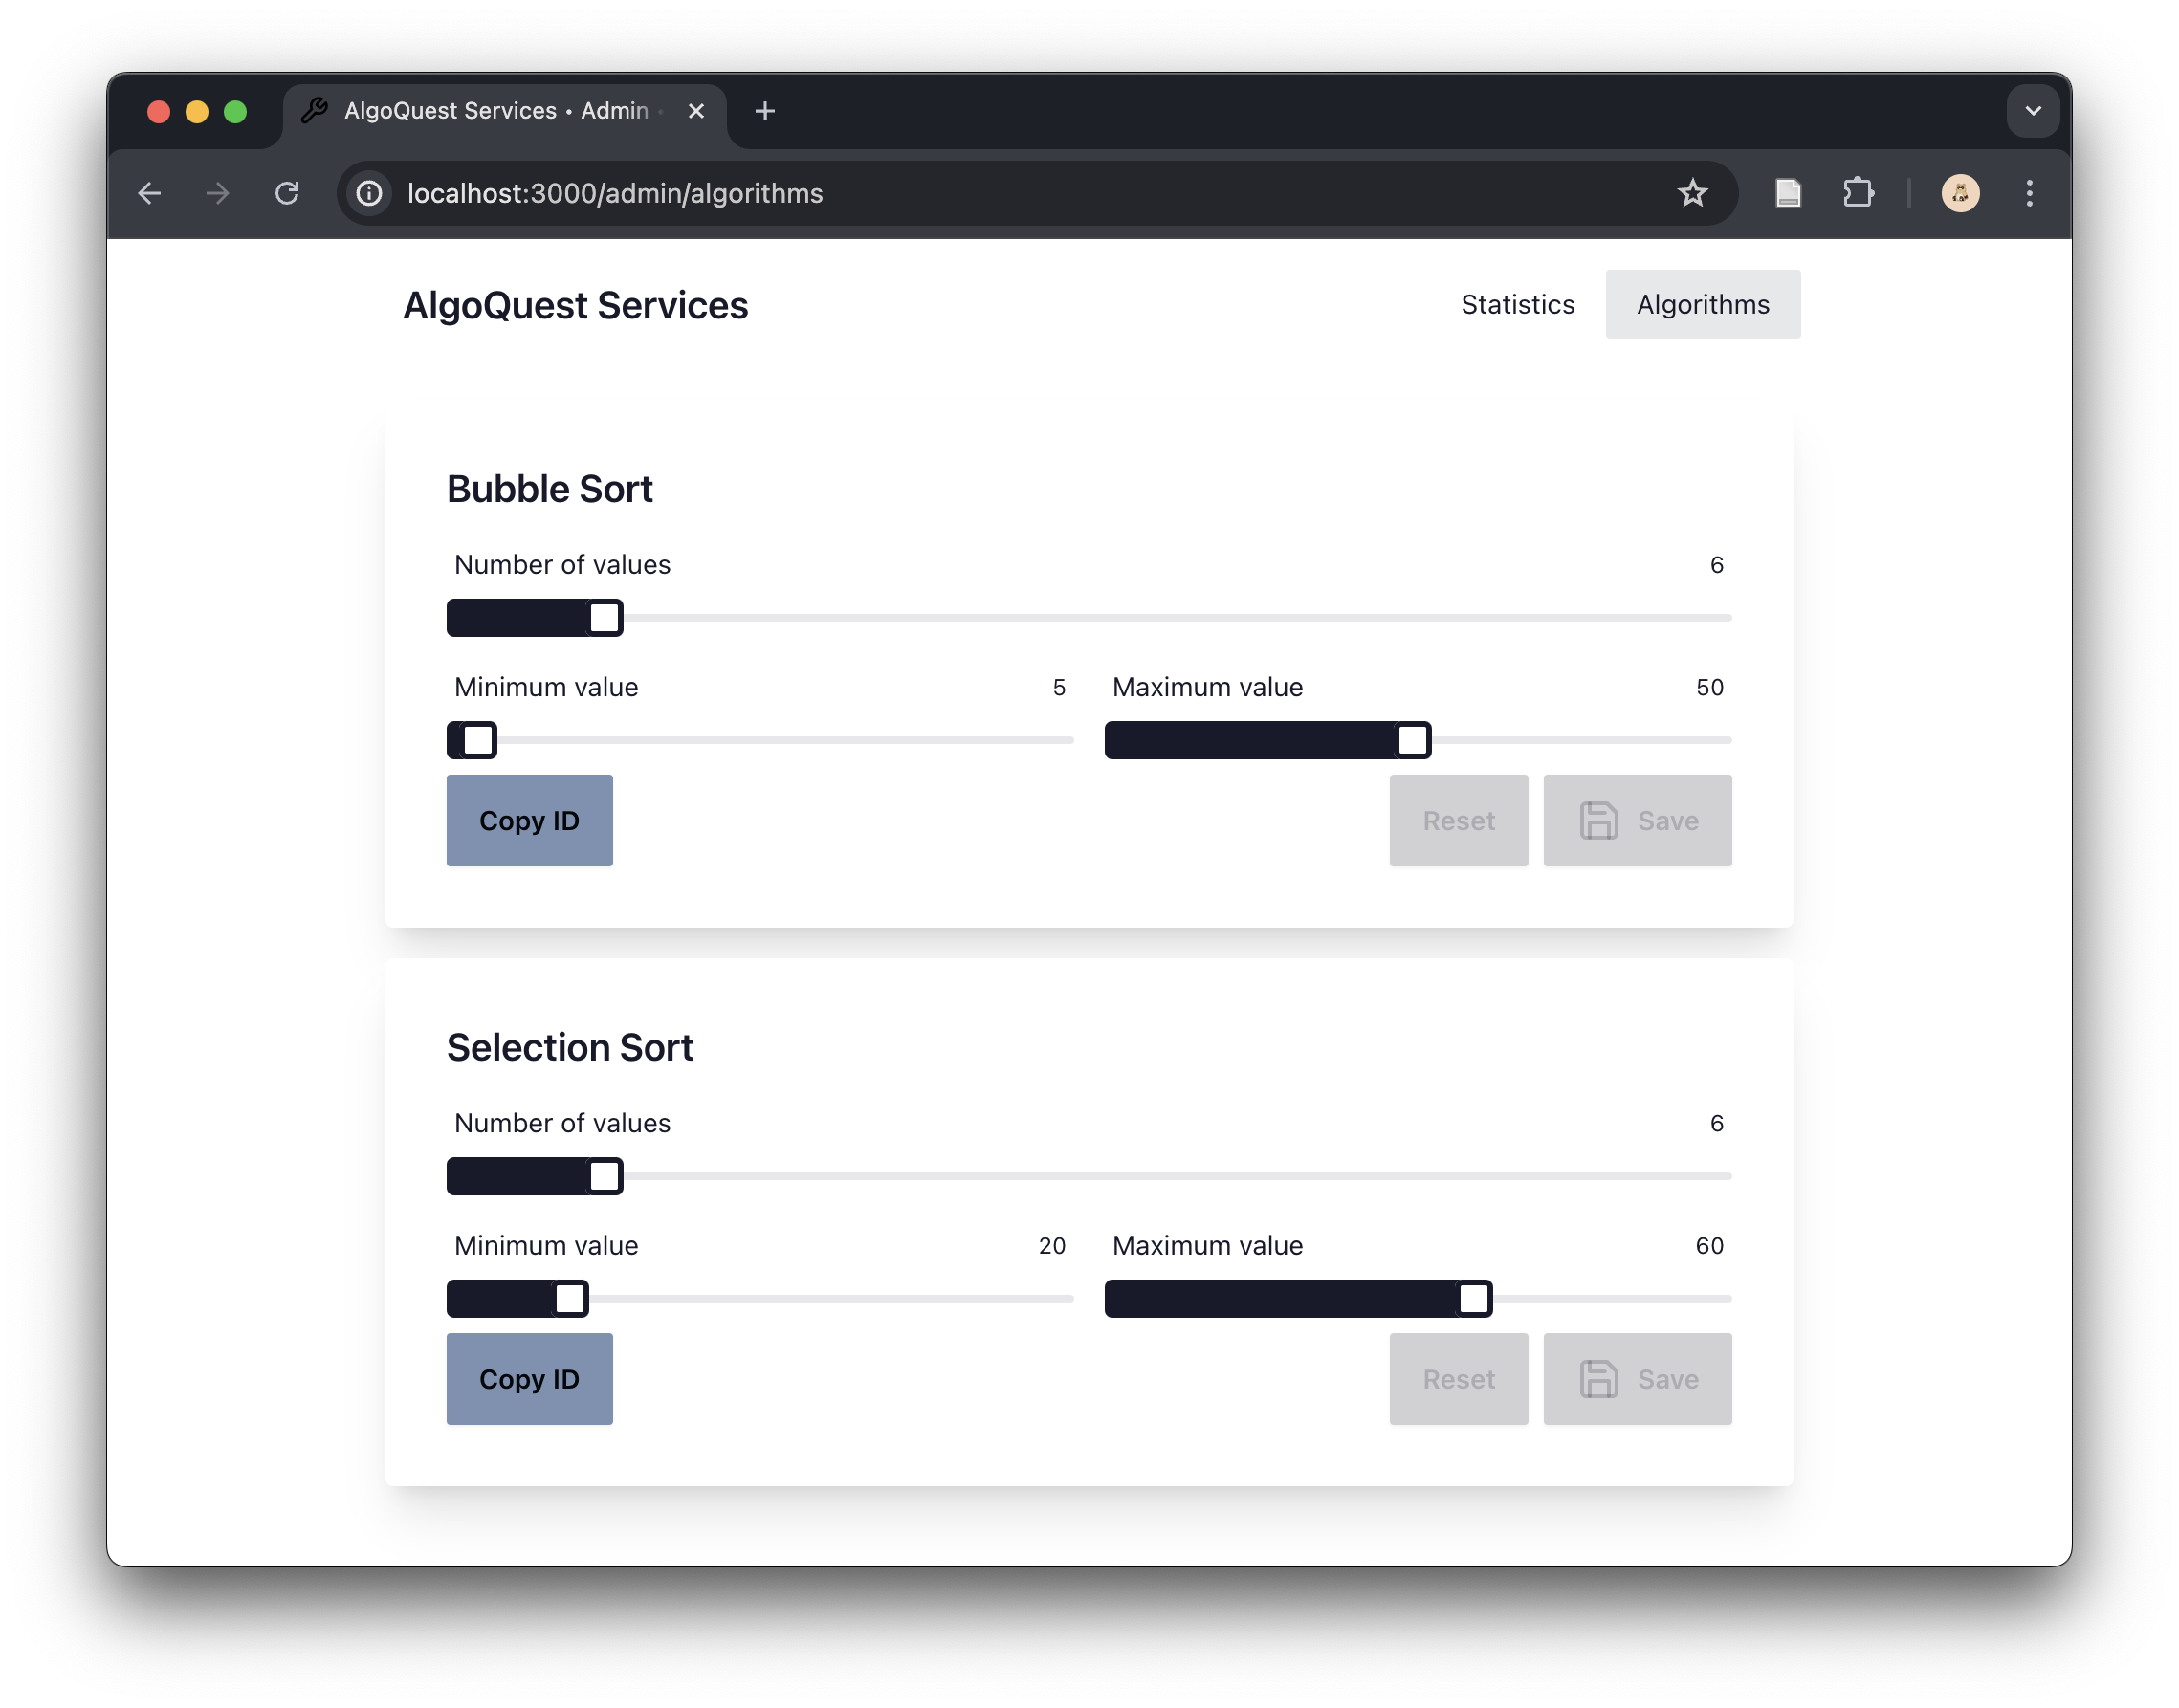
\includegraphics[width=0.7\linewidth]{sections/4/1/images/admin_dashboard_algorithm_config}
    \caption{Η σελίδα ρυθμίσεων των αλγορίθμων στο διαχειριστικό των εκπαιδευτικών}
    \label{fig:admin_dashboard_algorithm_config}
\end{figure}

Ο εκπαιδευτικός έχει πρόσβαση στη σελίδα ρυθμίσεων των αλγορίθμων (Εικόνα \ref{fig:admin_dashboard_algorithm_config}), όπου έχει τη δυνατότητα να ρυθμίσει τις παραμέτρους των αλγορίθμων που εμφανίζονται μέσα στο παιχνίδι. Το παιχνίδι, κατά την εκκίνηση του, διαβάζει τις τιμές που έχει θέσει ο εκπαιδευτικός και εκτελεί τις διαδικασίες του με βάση αυτές.

\begin{figure}[H]
    \centering
    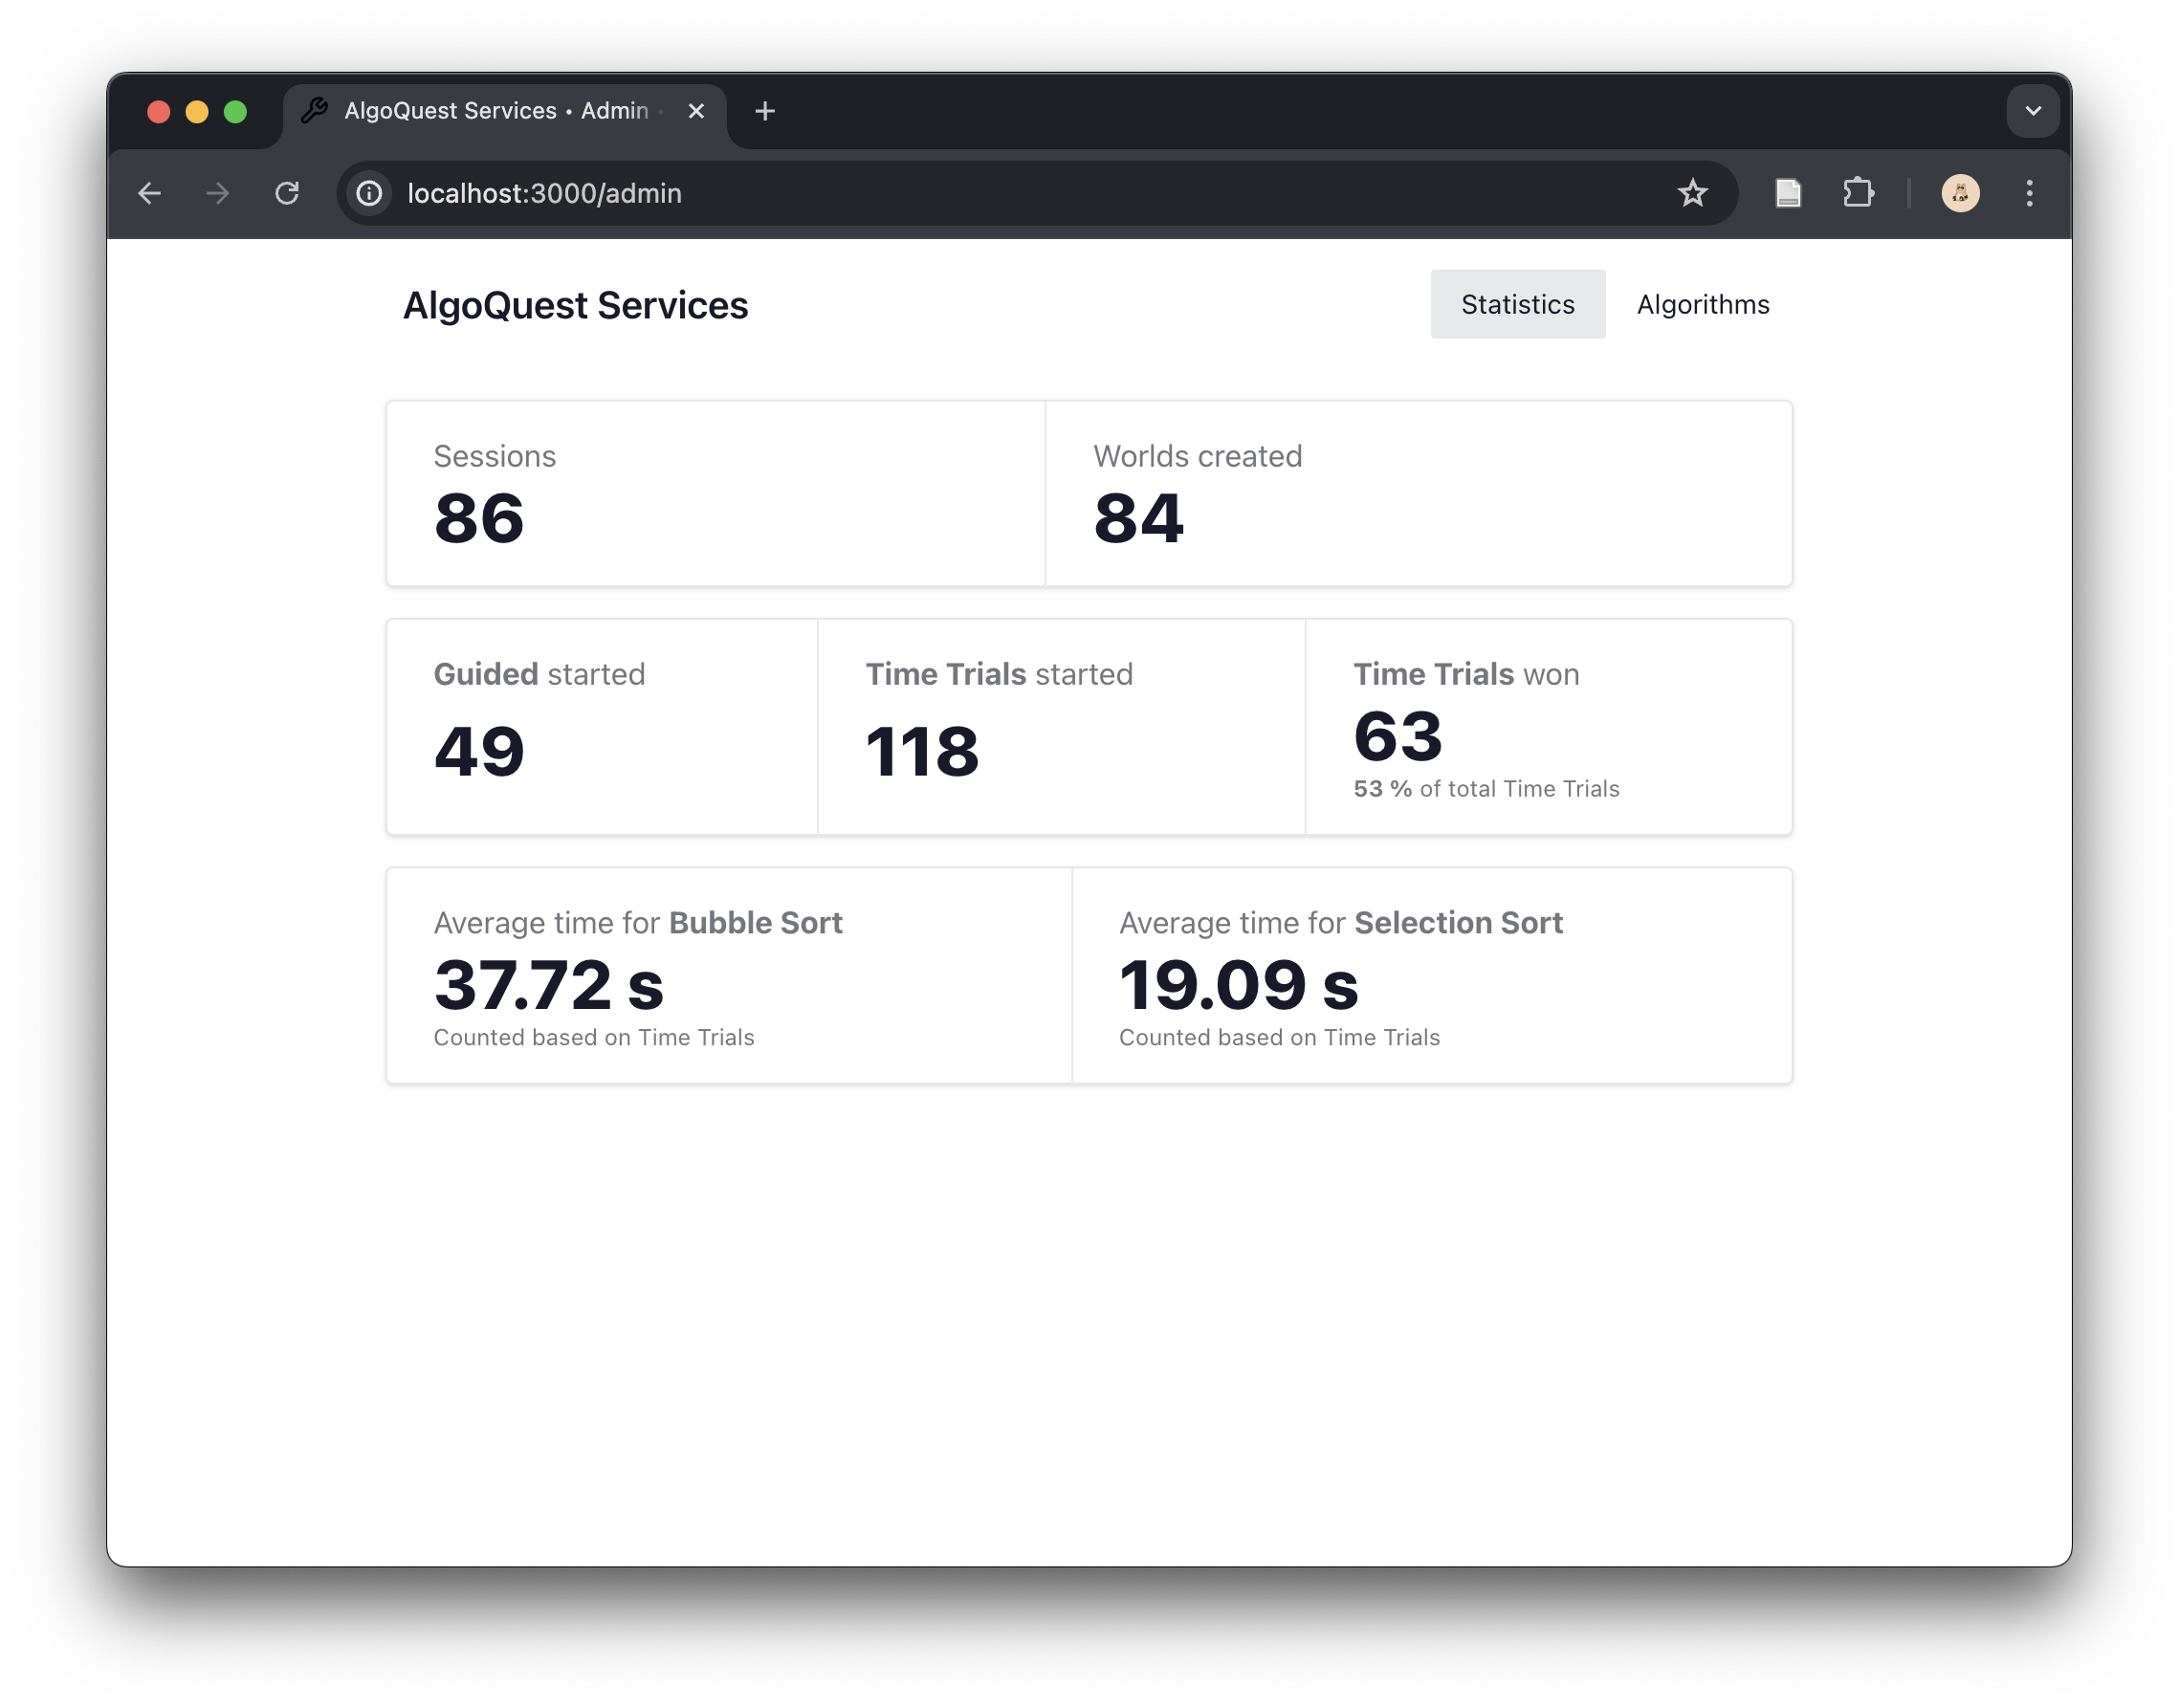
\includegraphics[width=0.7\linewidth]{sections/4/1/images/admin_dashboard_statistics}
    \caption{Η σελίδα στατιστικών στο διαχειριστικό των εκπαιδευτικών}
    \label{fig:admin_dashboard_statistics}
\end{figure}

Στη σελίδα στατιστικών (Εικόνα \ref{fig:admin_dashboard_statistics}) ο εκπαιδευτικός μπορεί με μια γρήγορη ματιά να δει γενικές και ενδιαφέρον πληροφορίες για το παιχνίδι. Η σελίδα αυτή μπορεί να εμπλουτιστεί με διάφορων ειδών στατιστικά που μπορούν να συλλεχθούν από την βάση δεδομένων.
